\documentclass[11pt,a4paper]{article}
\usepackage[margin=1in]{geometry}
\usepackage{graphicx}
\usepackage{booktabs}
\usepackage{amsmath}
\usepackage{float}
\usepackage{hyperref}
\usepackage{listings}
\usepackage{xcolor}

\lstset{basicstyle=\ttfamily\small,breaklines=true,frame=single,backgroundcolor=\color{gray!5}}

\title{\textbf{Auctions and Mechanism Design: Simulation Study}\\[4pt]
\large Second-Price Auction, First-Price Auction and VCG Mechanism}
\author{Sarah Fatima (B23EE1093)\\
Anshit Agarwal (B23CS1087)\\
Sahil Narkhede (B23CS1060)\\
Namya Dhingra (B23CS1040)}
\date{\today}

\begin{document}
\maketitle

\begin{abstract}
We simulate the second-price sealed-bid auction against three rival strategies, the first-price auction with $n=2,3,4$ bidders, and the VCG mechanism for procuring the cheapest path in a network. The results agree with theory: truthful bidding is a (weakly) dominant strategy in the second-price auction, the equilibrium bid $\frac{n-1}{n}v$ is the best response in the first-price auction, and truthful cost reporting is optimal in VCG. All code is in \texttt{auctions.py}.
\end{abstract}

%------------------------------------------------------------
\section{Part 1: Second-Price Sealed-Bid Auction}

\subsection{Setup}
Bidder 1 has a fixed value $v\in\{0.2,0.5,0.8\}$. Each rival draws a value $v_r\sim U[0,1]$ independently and uses one of three strategies: (a) \emph{truthful}, bid $v_r$; (b) \emph{half}, bid $v_r/2$; (c) \emph{random}, bid a fresh $U[0,1]$ draw, ignoring $v_r$.
Bidder 1 bids $b$. If $b$ exceeds the highest rival bid $p$, it wins, pays $p$ and gets utility $v-p$; otherwise its utility is $0$.
For each $v$, each strategy and each bid $b\in\{0.00,0.01,\dots,1.00\}$ we simulate $100{,}000$ auctions (fresh random draws for each bid) and average the utility. Ties have probability zero.

\subsection{Part A: one rival}
\begin{figure}[H]
\centering
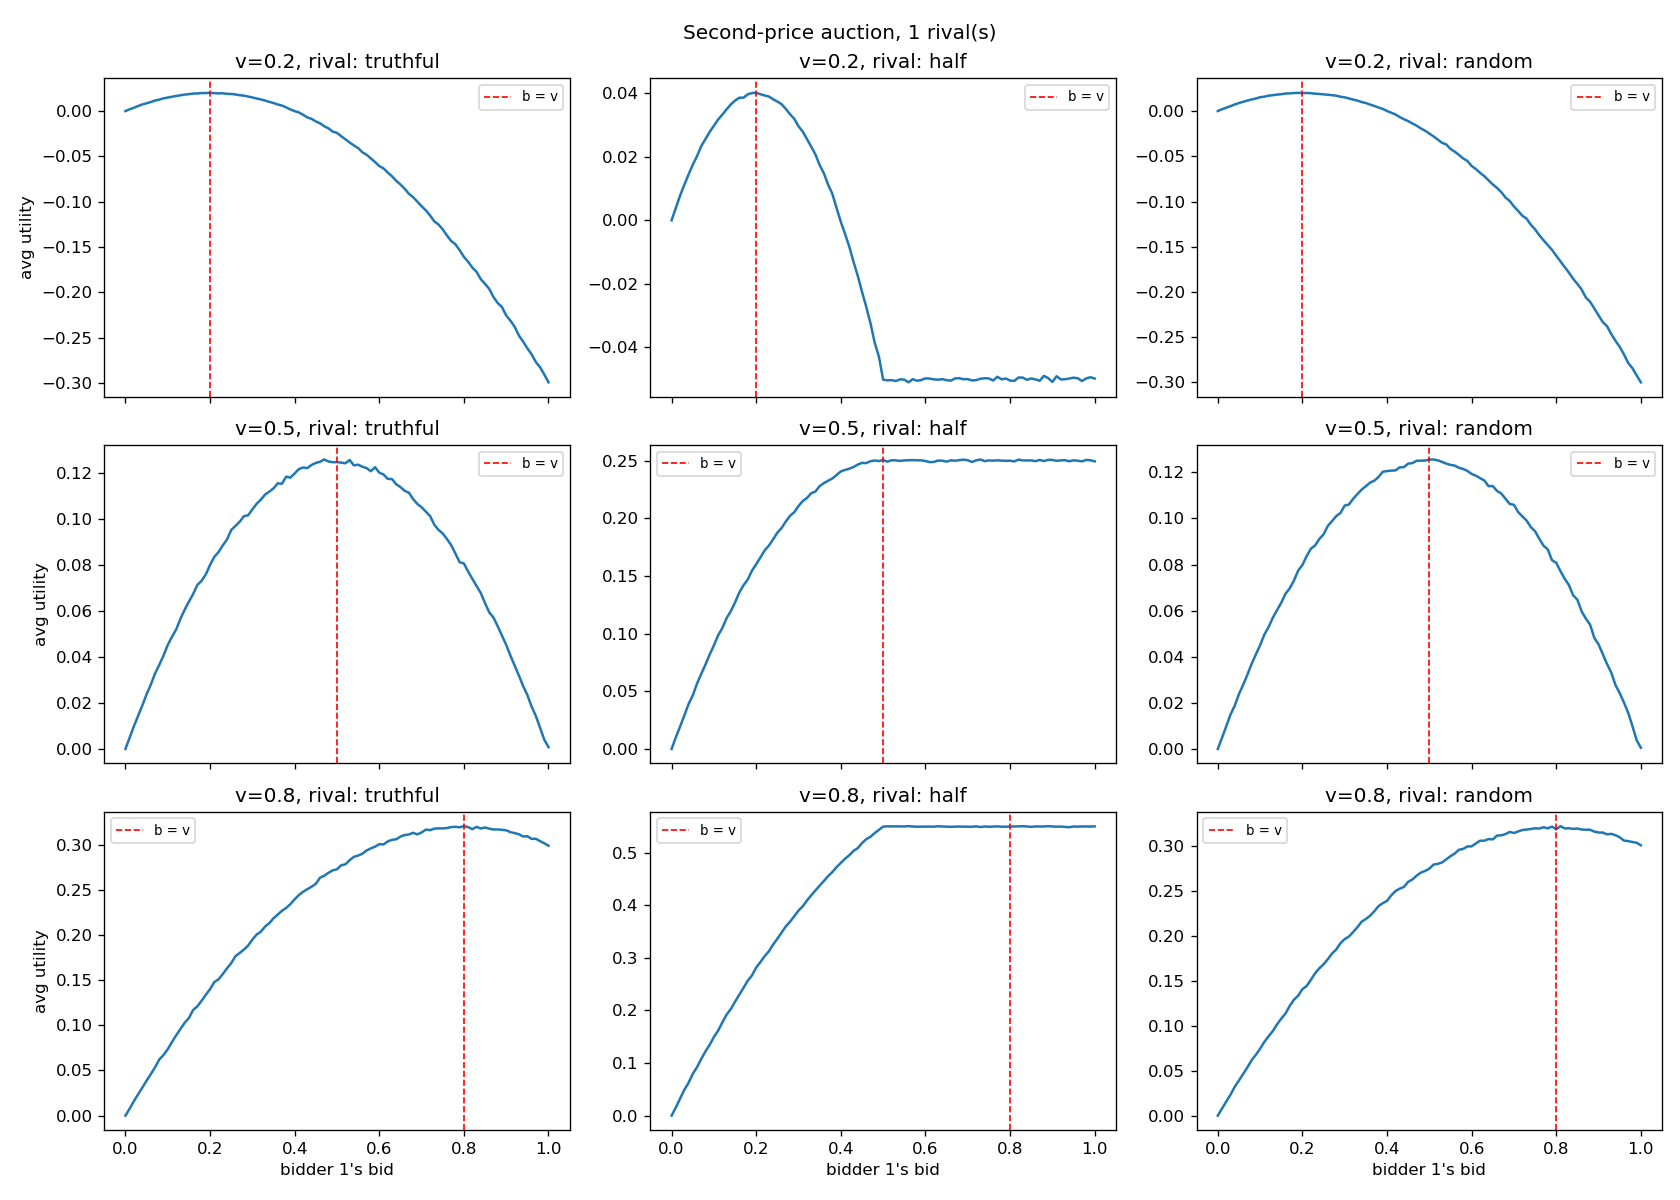
\includegraphics[width=\textwidth]{plots/part1A_1rivals.png}
\caption{Average utility of bidder 1 versus its bid, for each $v$ (rows) and rival strategy (columns). The dashed red line marks $b=v$.}
\label{fig:p1a}
\end{figure}

\begin{table}[H]
\centering
\begin{tabular}{llccc}
\toprule
$v$ & Rival & Best bid on grid & Max utility & $U(b=v)$\\
\midrule
0.2 & truthful & 0.20 & 0.0201 & 0.0201\\
0.2 & half     & 0.20 & 0.0402 & 0.0402\\
0.2 & random   & 0.19 & 0.0201 & 0.0199\\
0.5 & truthful & 0.47 & 0.1261 & 0.1249\\
0.5 & half     & 0.73 & 0.2510 & 0.2505\\
0.5 & random   & 0.51 & 0.1256 & 0.1256\\
0.8 & truthful & 0.80 & 0.3209 & 0.3209\\
0.8 & half     & 0.56 & 0.5507 & 0.5499\\
0.8 & random   & 0.81 & 0.3216 & 0.3181\\
\bottomrule
\end{tabular}
\caption{Part A results (one rival). Differences between the best bid and $v$ are within Monte-Carlo noise.}
\end{table}

\paragraph{Observations.}
Against truthful and random rivals the utility curve peaks at $b\approx v$. Against a rival bidding half its value, the curve is flat over a wide range of bids (about $0.5$--$1.0$ for $v=0.5,0.8$) because bidder 1 wins in nearly the same auctions and pays the same price for any bid in that range, so many bids tie with $b=v$. The simulated ``best'' bid (e.g.\ 0.73 for $v=0.5$) is therefore noise within a plateau.

\paragraph{Do the plots help bidder 1 choose a strategy?}
Partly. They show empirically that no bid does noticeably better than $b=v$ against any of the three rival strategies, even though bidder 1 does not know the rival's strategy. They do not explain this: the plots are averages over a specific rival distribution and are noisy, and the flat regions give no unique best bid. The dominance argument in Part B is what justifies truthful bidding, and the plots are consistent with it.

\subsection{Part B: fixed rival bids}
Let the rival bid be fixed at $p\in\{0.1,0.4,0.9\}$. Utility of bidder 1 is $v-p$ if $b>p$ and $0$ otherwise. We evaluated it for every $b$ on the grid:

\begin{table}[H]
\centering
\begin{tabular}{cccccc}
\toprule
Rival bid $p$ & $v$ & $U(b=v)$ & $\max_b U(b)$ & $b=v$ optimal?\\
\midrule
0.1 & 0.2 & 0.10 & 0.10 & yes\\
0.1 & 0.5 & 0.40 & 0.40 & yes\\
0.1 & 0.8 & 0.70 & 0.70 & yes\\
0.4 & 0.2 & 0.00 & 0.00 & yes\\
0.4 & 0.5 & 0.10 & 0.10 & yes\\
0.4 & 0.8 & 0.40 & 0.40 & yes\\
0.9 & 0.2 & 0.00 & 0.00 & yes\\
0.9 & 0.5 & 0.00 & 0.00 & yes\\
0.9 & 0.8 & 0.00 & 0.00 & yes\\
\bottomrule
\end{tabular}
\caption{Part B: $b=v$ attains the maximum utility in all nine cases.}
\end{table}

\paragraph{Why.} If $v>p$, any bid $b>p$ wins and pays $p$, so $b=v$ achieves the maximum $v-p$. If $v<p$, winning would give $v-p<0$, and $b=v$ loses and gets $0$. If $v=p$, utility is $0$ either way. Hence $b=v$ is weakly dominant: no other bid gives strictly higher utility against any rival bid. (Other bids can tie with $b=v$, which is why the optimum is not unique.)

\subsection{Part C: two rivals}
Bidders 2 and 3 both draw $U[0,1]$ values and use the \emph{same} strategy. Bidder 1 wins if its bid exceeds the maximum of the two rival bids and pays that maximum. Parts A and B are repeated. For Part B we used rival bid pairs $(0.1,0.4)$, $(0.4,0.9)$, $(0.1,0.9)$, and $b=v$ was again optimal in all cases.

\begin{figure}[H]
\centering
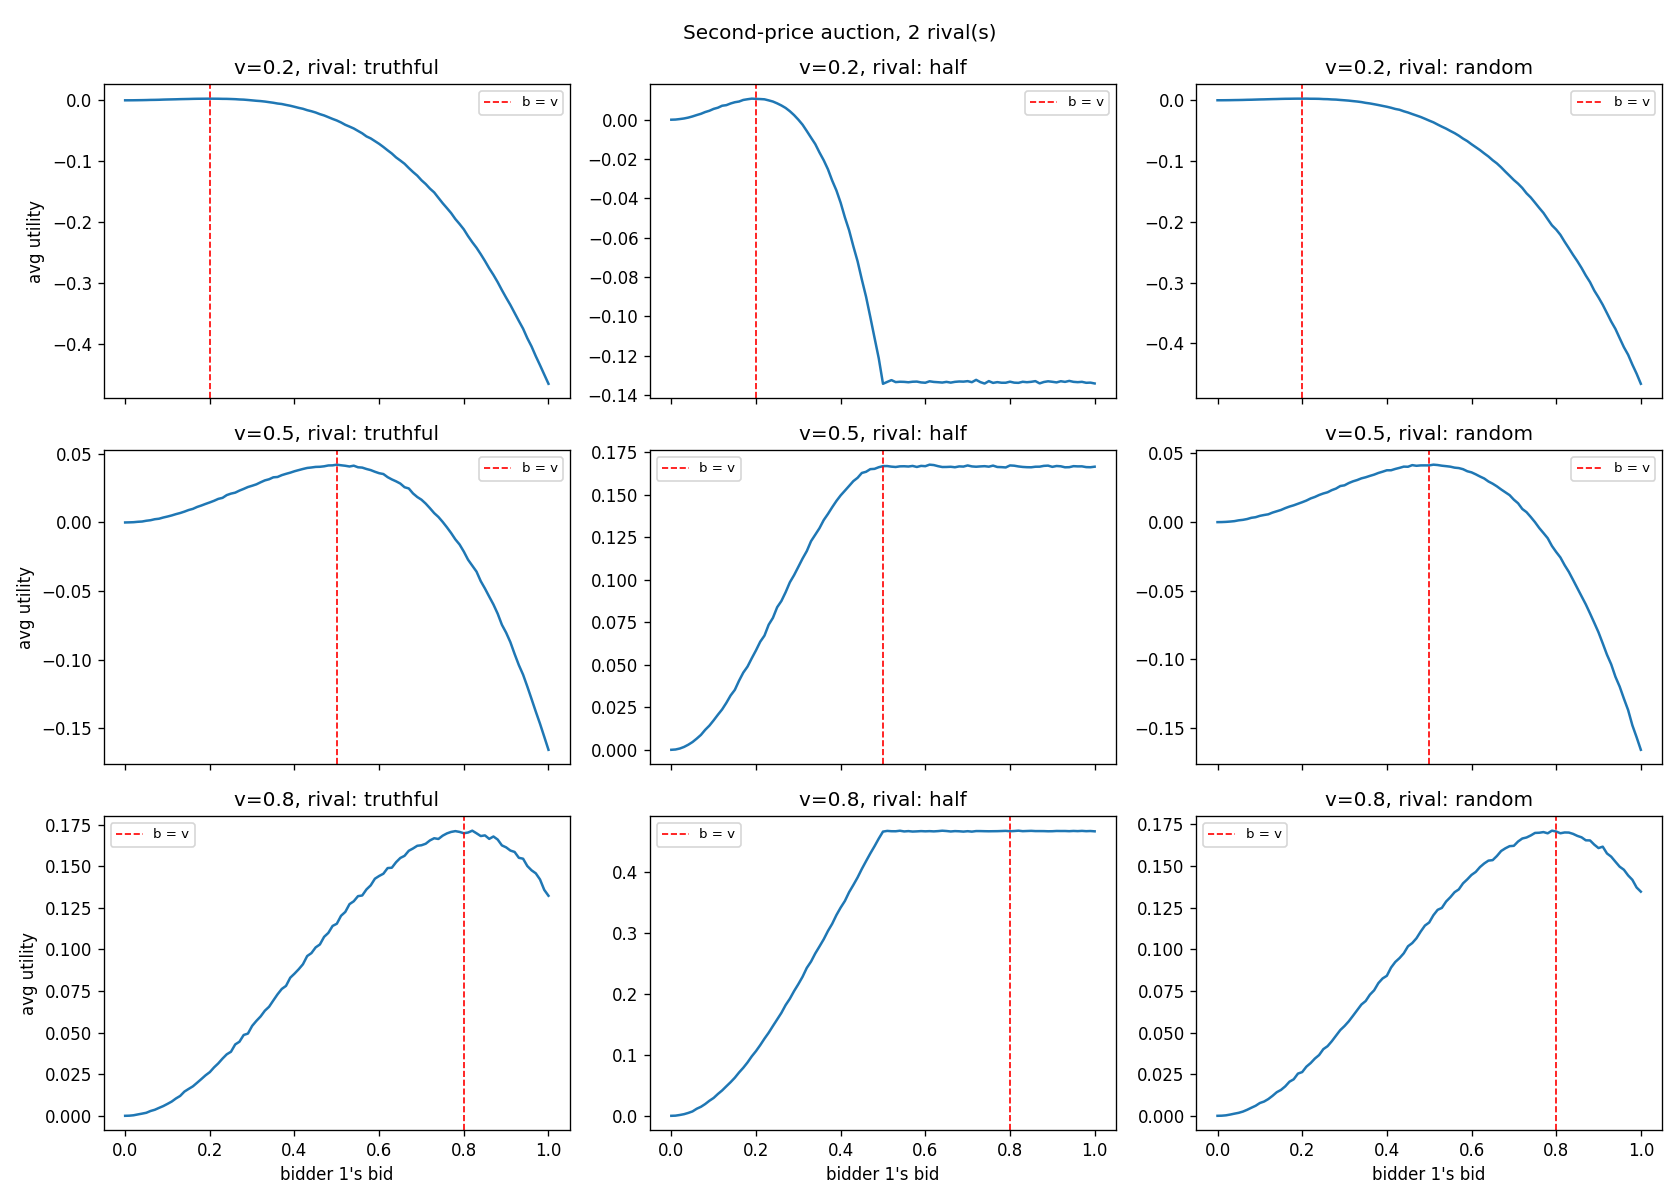
\includegraphics[width=\textwidth]{plots/part1C_2rivals.png}
\caption{Same as Figure~\ref{fig:p1a} with two rivals using the same strategy.}
\end{figure}

\begin{table}[H]
\centering
\begin{tabular}{llccc}
\toprule
$v$ & Rival strategy & Best bid on grid & Max utility & $U(b=v)$\\
\midrule
0.2 & truthful & 0.20 & 0.0027 & 0.0027\\
0.2 & half     & 0.19 & 0.0107 & 0.0106\\
0.2 & random   & 0.19 & 0.0026 & 0.0026\\
0.5 & truthful & 0.50 & 0.0422 & 0.0422\\
0.5 & half     & 0.61 & 0.1678 & 0.1669\\
0.5 & random   & 0.51 & 0.0419 & 0.0413\\
0.8 & truthful & 0.82 & 0.1714 & 0.1698\\
0.8 & half     & 0.82 & 0.4675 & 0.4665\\
0.8 & random   & 0.79 & 0.1712 & 0.1706\\
\bottomrule
\end{tabular}
\caption{Part C results. Utilities are lower than with one rival because the price is the maximum of two rival bids.}
\end{table}

The conclusions of Part A and B carry over. The optimum remains at or near $b=v$ (with a plateau against half-value rivals), and expected utility falls as more rivals are added.

%------------------------------------------------------------
\section{Part 2: First-Price Auction with $n$ Bidders}

\subsection{Setup}
All $n$ valuations are i.i.d.\ $U[0,1]$. Bidders $2,\dots,n$ bid the equilibrium bid $\frac{n-1}{n}v_i$. Bidder 1 bids $k\,v_1$ for $k\in\{0.1,0.2,\dots,2.0\}$. The winner pays its own bid. For each $k$ we simulate $100{,}000$ auctions and estimate (i) the expected utility of bidder 1 (averaged over its random valuation) and (ii) the fraction of auctions in which the winner, whoever it is, could have paid less and still won, i.e.\ winning bid $>$ second-highest bid. We also record the average gap between the two highest bids.

\begin{figure}[H]
\centering
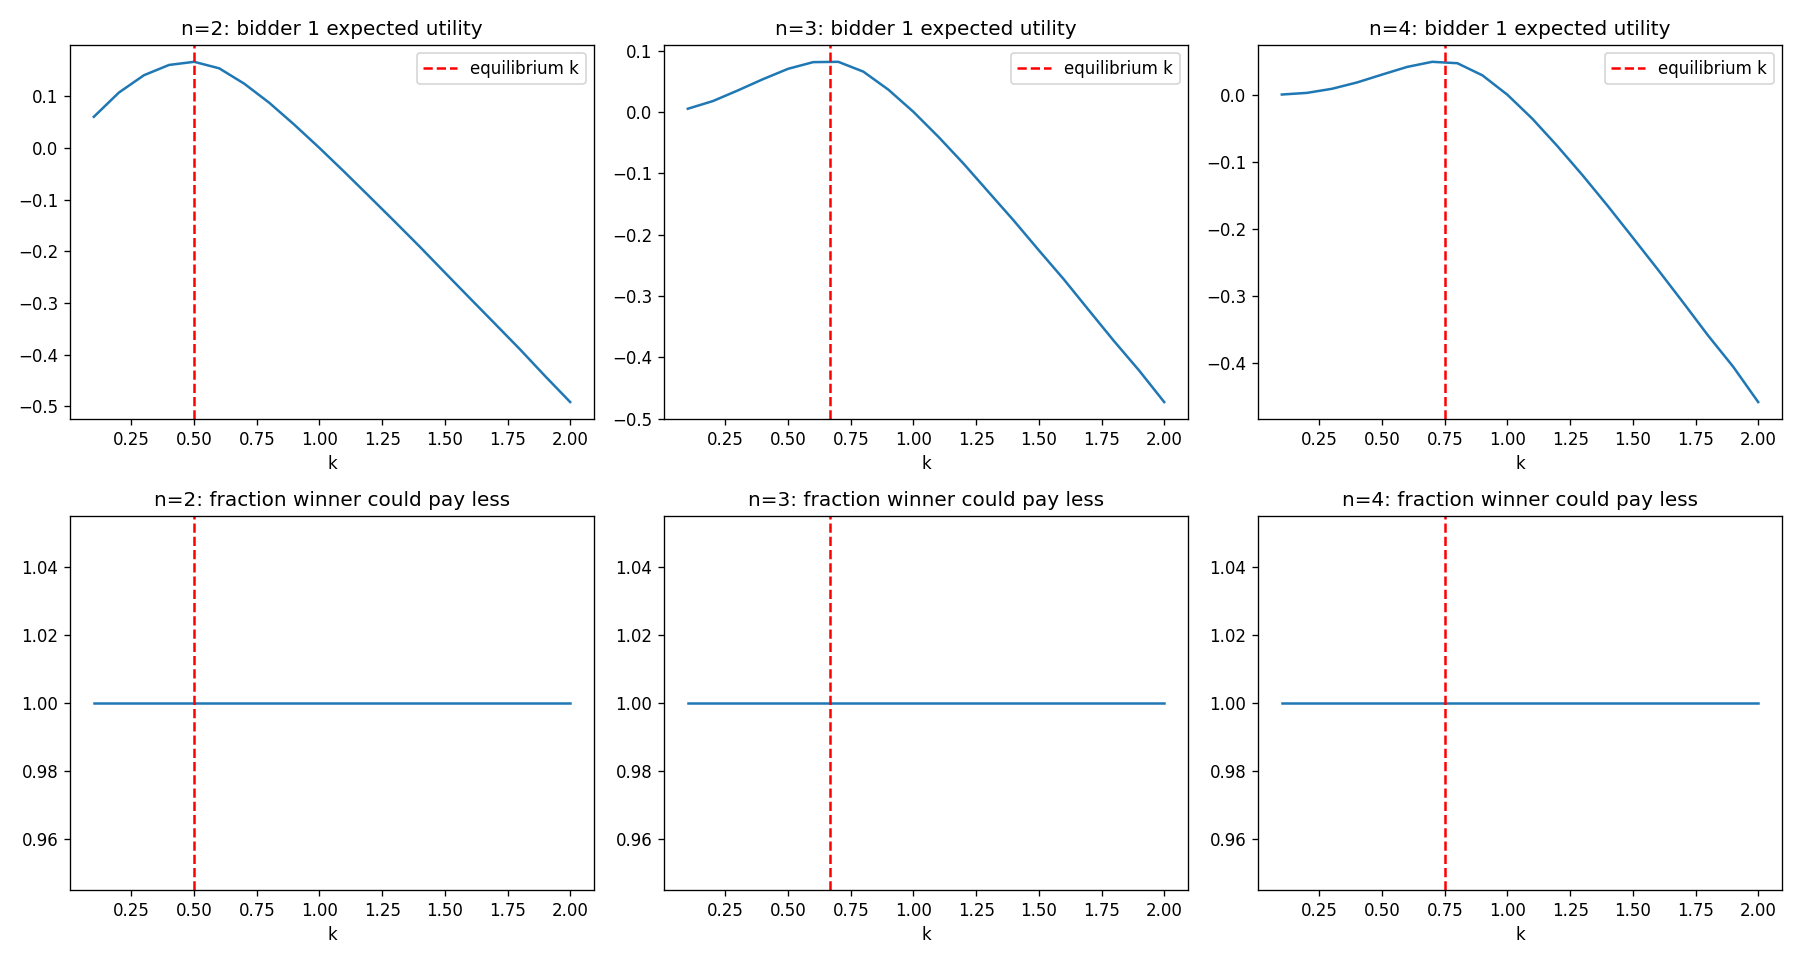
\includegraphics[width=\textwidth]{plots/part2_first_price.png}
\caption{Top row: expected utility of bidder 1 versus $k$ for $n=2,3,4$ (red dashed line: equilibrium $k=\frac{n-1}{n}$). Bottom row: fraction of auctions where the winner could have paid less.}
\end{figure}

\begin{table}[H]
\centering
\begin{tabular}{ccccccc}
\toprule
$n$ & Equilibrium $k$ & Best $k$ on grid & Max $U_1$ & $U_1(k{=}1)$ & Fraction winner could pay less\\
\midrule
2 & 0.500 & 0.5 & 0.1667 & 0.0000 & 1.000\\
3 & 0.667 & 0.7 & 0.0816 & 0.0000 & 1.000\\
4 & 0.750 & 0.7 & 0.0492 & 0.0000 & 1.000\\
\bottomrule
\end{tabular}
\caption{Part 2 summary. For $n=4$ the equilibrium $k=0.75$ lies between grid points $0.7$ and $0.8$ ($U_1=0.0492$ and $0.0471$).}
\end{table}

\begin{table}[H]
\centering
\begin{tabular}{ccccccc}
\toprule
$k$ & \multicolumn{2}{c}{$n=2$} & \multicolumn{2}{c}{$n=3$} & \multicolumn{2}{c}{$n=4$}\\
 & $U_1$ & avg gap & $U_1$ & avg gap & $U_1$ & avg gap\\
\midrule
0.3 & 0.1408 & 0.1598 & 0.0350 & 0.1930 & 0.0090 & 0.1792\\
0.5 & 0.1667 & 0.1666 & 0.0702 & 0.1680 & 0.0302 & 0.1622\\
0.7 & 0.1244 & 0.2188 & 0.0816 & 0.1702 & 0.0492 & 0.1490\\
0.8 & 0.0873 & 0.2546 & 0.0656 & 0.1866 & 0.0471 & 0.1541\\
1.0 & 0.0000 & 0.3344 & 0.0000 & 0.2420 & 0.0000 & 0.1909\\
1.5 & $-0.2410$ & 0.5560 & $-0.2255$ & 0.4300 & $-0.2131$ & 0.3567\\
\bottomrule
\end{tabular}
\caption{Expected utility of bidder 1 and average gap between the two highest bids, for selected $k$.}
\end{table}

\paragraph{Observations.}
\begin{itemize}
\item Bidder 1's utility is maximised at (or next to) the equilibrium multiplier $\frac{n-1}{n}$. Bidding too low loses profitable auctions; bidding too high wins more but pays too much. At $k=1$ (bidding the true value) the utility is zero, and for $k>1$ it is negative.
\item As $n$ grows, the optimal shading shrinks ($k\to1$) and expected utility falls, since competition is stiffer.
\item The fraction of auctions where the winner could have paid less is essentially $1$ for every $k$ and $n$: bids are continuous, so the top two bids almost never coincide. The first-price auction therefore always leaves some money on the table, with average gap between the top two bids of roughly $0.15$--$0.17$ at equilibrium. This is unlike the second-price auction, where the winner pays exactly the second-highest bid.
\end{itemize}

%------------------------------------------------------------
\section{Part 3: VCG Mechanism for the Cheapest Path}

\subsection{Setup}
Each edge is an agent with a private cost $c_e$. The mechanism picks the cheapest path from A to F (brute-force over all simple paths). The VCG payment to a chosen edge $e$ is
\[
p_e = C(G\setminus e) - \bigl(C(P^*) - c_e\bigr),
\]
where $C(G\setminus e)$ is the cheapest path cost when $e$ is removed and $C(P^*)$ is the cost of the chosen path. Edges not on the chosen path are paid $0$. The utility of an edge is $p_e-c_e$ if chosen and $0$ otherwise.

\paragraph{Graph used.} We could not directly verify Figure 7.3, so we used costs consistent with the payments stated in the text: AB$=3$, BE$=1$, EF$=2$ on the cheapest path (cost 6) and an alternative path A--C--D--F with AC$=2$, CD$=3$, DF$=2$ (cost 7). If the book's costs differ, the \texttt{COSTS} dictionary in the code can be changed.

\subsection{Result}
\begin{table}[H]
\centering
\begin{tabular}{lcc}
\toprule
Edge & Cost & VCG payment\\
\midrule
AB & 3 & 4\\
BE & 1 & 2\\
EF & 2 & 3\\
AC, CD, DF & 2, 3, 2 & 0\\
\bottomrule
\end{tabular}
\caption{The chosen path is ABEF (cost 6); payments match the text.}
\end{table}

\subsection{Misreporting}
We chose BE (on the path, true cost 1) and CD (off the path, true cost 3) and let each report every cost from $0$ to $10$ in steps of $0.5$, with the others truthful. Utility is always computed using the \emph{true} cost.

\begin{figure}[H]
\centering
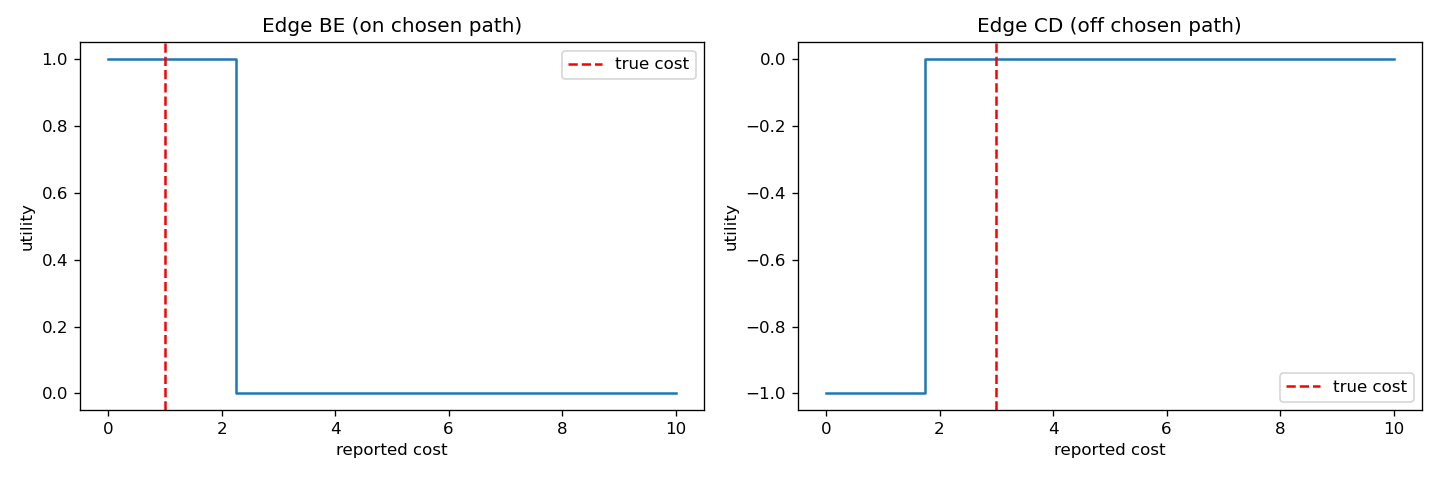
\includegraphics[width=0.95\textwidth]{plots/part3_vcg.png}
\caption{Utility versus reported cost for BE (left) and CD (right). Red dashed line: true cost.}
\end{figure}

\begin{itemize}
\item \textbf{BE (on path):} the utility is $1$ for any report up to $2$ and drops to $0$ for higher reports, since BE then drops out of the cheapest path. The payment does not depend on the report as long as the edge stays on the path, so lying cannot raise it. Truthful reporting is optimal.
\item \textbf{CD (off path):} the utility is $0$ for every report from $2$ to $10$. Reporting below $2$ would put CD on the winning path but at a payment below its true cost, giving negative utility. No misreport helps.
\end{itemize}
Thus truthful reporting is a dominant strategy for both edges, as VCG guarantees.

%------------------------------------------------------------
\section{Conclusion}
The simulations confirm three standard results: (i) truthful bidding is weakly dominant in the second-price auction, whatever the rivals do; (ii) in the first-price auction the best response to equilibrium bidders is to shade the bid by $\frac{n-1}{n}$, and the winner almost always could have paid less; (iii) VCG makes truthful reporting optimal for every edge, and reproduces the payments (4, 2, 3) from the text.

\appendix
\section{Code}
The full implementation is in \texttt{auctions.py}, run with \texttt{python auctions.py}. It uses NumPy and Matplotlib, with a fixed random seed (42) for reproducibility, and saves the figures to \texttt{plots/}.

\end{document}